\documentclass[hidelinks,12pt]{article}
\usepackage[utf8]{inputenc}
\usepackage[table,xcdraw]{xcolor}
\usepackage{mathtools}
\usepackage{amsthm}
\usepackage{amsmath}
\usepackage{amsfonts}
\usepackage{amssymb}
\usepackage{centernot}
\usepackage{marvosym}
\usepackage{enumitem}
\usepackage{hyperref}
\setcounter{tocdepth}{1}
\let\marvosymLightning\Lightning
\newtheorem{theorem}{Theorem}
\newtheorem{corollary}{Corollary}[theorem]
\newtheorem*{remark}{Remark}
\renewcommand\qedsymbol{QED}
\newcommand{\C}{\mathbb{C}}
\newcommand{\R}{\mathbb{R}}
\newcommand{\N}{\mathbb{N}}
\newcommand{\Z}{\mathbb{Z}}
\newcommand{\divby}{%
  \mathrel{\text{\vbox{\baselineskip.65ex\lineskiplimit0pt\hbox{.}\hbox{.}\hbox{.}}}}%
  }
\newcommand{\notdivby}{\centernot\divby}
\title{\scalebox{2}{Math 531 Homework 3}}
\author{\scalebox{1.5}{Theo Koss}}
\date{February 2021}
\begin{document}
\graphicspath{{/home/theo/Documents/GitHub/Math-Homeworks/Math 531/Random/}}
\maketitle
\section{Section 2.1}
\begin{itemize}
    \item Problem 1:\begin{enumerate}[label=(\alph*)]
        \item $f:\R\to\R;f(x)=x+3$.
        \newline Injective and surjective. This is a bijection
        \item $f:\C\to\C;f(x)=x^2+2x+1$.\newline Surjective but not injective.
        \item $f:\Z_n\to\Z_n;f([x]_n)=[mx+b]_n,$ where $m,b\in\Z$.\newline Neither injective nor surjective? (What if $m,b=0$).
        \item $f:\R^+\to\R;f(x)=ln(x)$.\newline Injective and surjective. This is a bijection.
    \end{enumerate}
    \item Problem 6: Let $S=\{1,2,3\}$ and $T=\{4,5\}$.\begin{enumerate}[label=(\alph*)]
    \item How many functions are there from $S\to T$? From $T\to S$?\newline There are $2^3=8$ from $S\to T$, and $3^2=9$ from $T\to S$.
    \item How many of the functions from $S\to T$ are one-to-one? How many are onto?\newline None of the functions are one-to-one. There are 6 functions that are onto.
    \item How many of the functions from $T\to S$ are one-to-one? How many are onto?\newline There are 6 functions from $T\to S$ that are one-to-one. None of the functions are onto.
    \end{enumerate}
    \item Problem 15: Let $f:A\to B$ and $g:B\to C$ be functions. Prove that if $g\circ f$ is one-to-one, the $f$ is one-to-one, and that if $g\circ f$ is onto, then $g$ is onto. \begin{proof}
    Consider $A=\{x_1,x_2,x_3,...,x_n\}$, $B=\{y_1,y_2,y_3,...,y_n\}$ and $C=\{z_1,z_2,z_3,...,z_n\}$. Since $g\circ f$ is one-to-one, 
    \end{proof}
\end{itemize}
\section{Section 2.2}
\begin{itemize}
    \item Problem 4: Let $S$ be the set of all ordered pairs $(m,n)$ of positive integers. For $(a_1,a_2)\in S$ and $(b_1,b_2)\in S$, define $(a_1,a_2)\sim(b_1,b_2)$ if $a_1+b_2=a_2+b_1.$ Show that $\sim$ is an equivalence relation.\begin{proof}
    Reflexivity: Check $(a,b)\sim (a,b)\Longrightarrow a+b=a+b$.
    \newline Symmetry: Check $(a,b)\sim (c,d)$ iff $(c,d)\sim(a,b)$. Then $a+b=c+d$ iff $c+d=a+b$. This is true.
    \newline Transitivity: Check if $(a,b)\sim (c,d)$ and $(c,d)\sim(e,f)$, then $(a,b)\sim(e,f)$.
    \newline $a+b=c+d$ and $c+d=e+f$, so we can replace $c+d$ in the second equation to get: $a+b=e+f$. Then $(a,b)\sim(e,f)$. Therefore this is an equivalence relation.
    \end{proof}
    \item Problem 9: Show that any circular relation is an equivalence relation. \begin{proof}
    By definition, $R\subseteq S\times S$ is both symmetric and transitive. (IDK how to show reflexivity? I think it has to do with the fact that transitivity is stronger than reflexivity but idk)
    \end{proof}
\end{itemize}
\section{Section 2.3}
\begin{itemize}
    \item Problem 3: $\left(\begin{smallmatrix} 
1&2&3&4&5&6&7&8&9&10\\
3&4&10&5&7&8&2&6&9&1
\end{smallmatrix}\right)$ As a product of disjoint cycles and as a product of transpositions, construct its associated diagram, and find its order.\newline $\left(\begin{smallmatrix} 
1&2&3&4&5&6&7&8&9&10\\
3&4&10&5&7&8&2&6&9&1
\end{smallmatrix}\right)$=$\left(\begin{smallmatrix} 
1&3&10&2&4&5&7&6&8&9\\
3&10&1&4&5&7&2&8&6&9
\end{smallmatrix}\right)$=$\left(\begin{smallmatrix} 
1&3&10\\
3&10&1
\end{smallmatrix}\right)\cdot\left(\begin{smallmatrix} 
2&4&5&7\\
4&5&7&2
\end{smallmatrix}\right)\cdot\left(\begin{smallmatrix} 
6&8\\
8&6
\end{smallmatrix}\right)\cdot\left(\begin{smallmatrix} 
9\\
9
\end{smallmatrix}\right)$\newline\scalebox{.15}{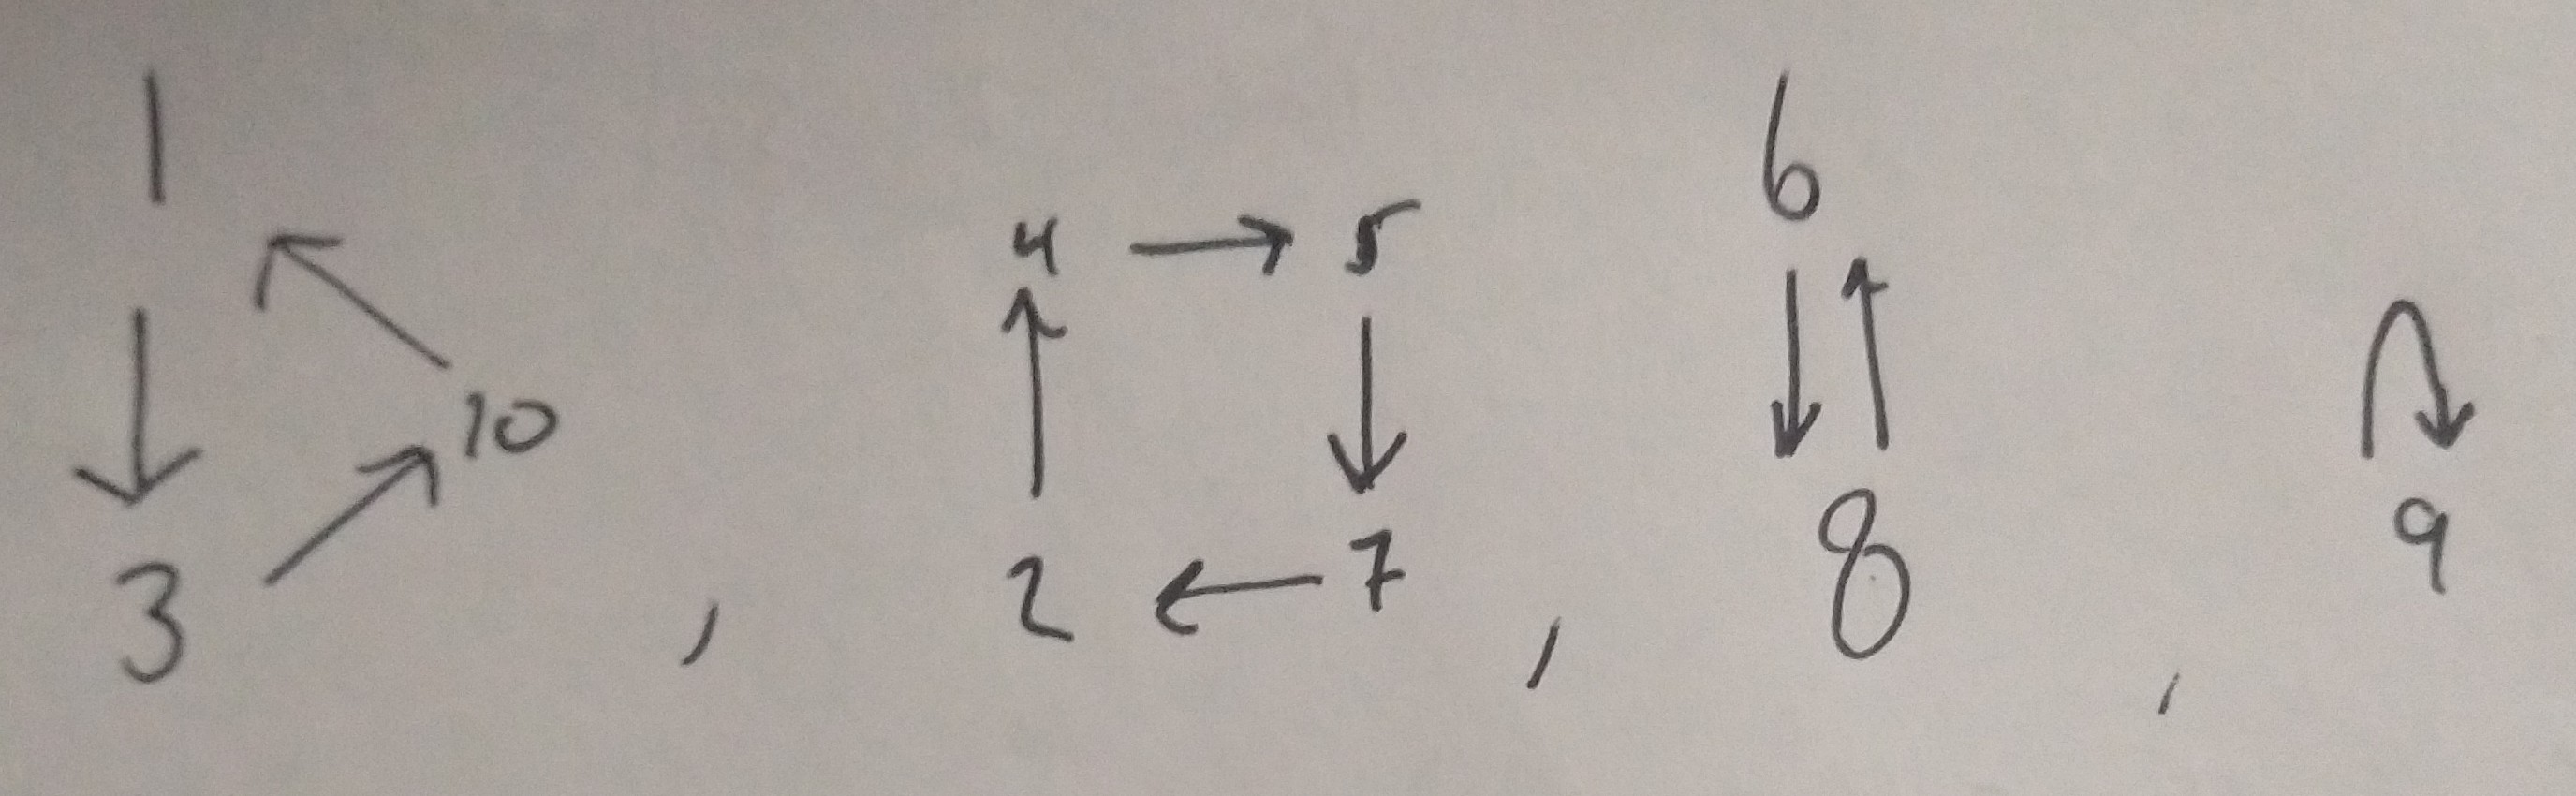
\includegraphics{Cyclediagram}}\newline The order is 12.
    \item Problem 7: Not sure :/
    \item Problem 14: Prove that $(a,b)$ cannot be written as a product of two cycles of length three. \begin{proof}
    $(a,b)$ is an odd permutation. A cycle of length 3 is an even permutation, and even times even can never be odd, therefore the product of two cycles of length 3 is even.
    \end{proof}
\end{itemize}
\end{document}
